% -- Encoding UTF-8 without BOM
% -- XeLaTeX => PDF (BIBER)

\documentclass[espanol]{cv-style}          % Add 'print' as an option into the square bracket to remove colours from this template for printing. 
                                    % Add 'espanol' as an option into the square bracket to change the date format of the Last Updated Text

\sethyphenation{spanish}{PostgreSQL contribuyentes Nacional identificación bajo} % Add words between the {} to avoid them to be cut 
\exhyphenpenalty=10000
\hyphenpenalty=10000
\begin{document}

\header{Meili }{Vanegas-Hernandez}           % Your name
\lastupdated

%----------------------------------------------------------------------------------------
%	SIDEBAR SECTION  -- In the aside, each new line forces a line break
%----------------------------------------------------------------------------------------

\begin{aside}
%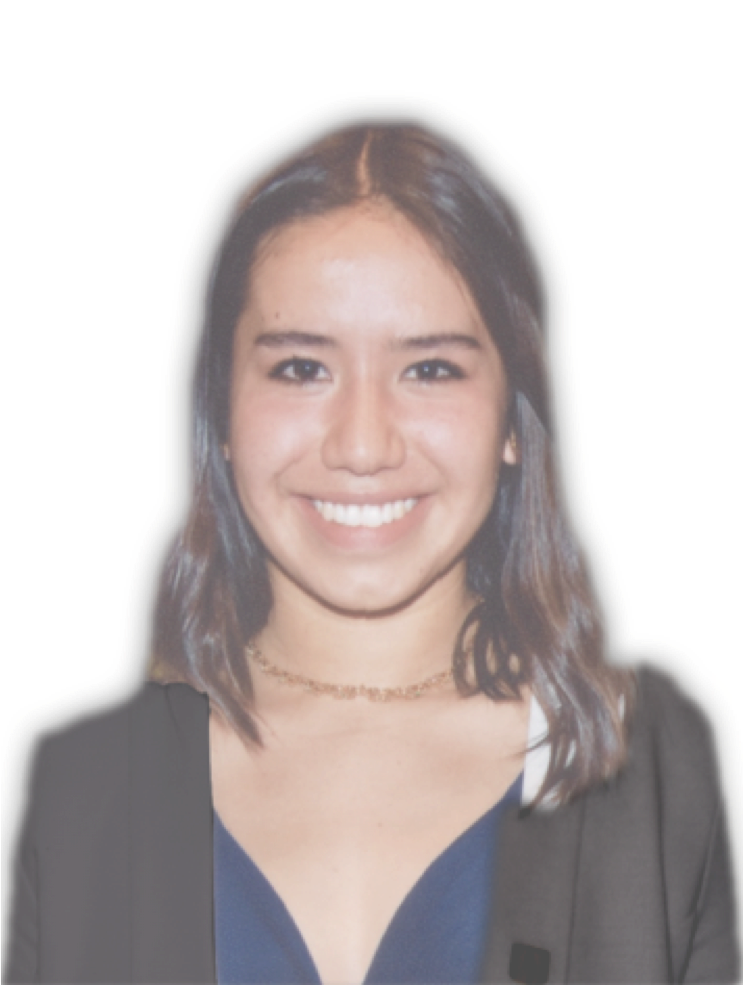
\includegraphics[width=3cm]{pictures/me.png}
%
\vspace{2.5cm}
\section{\textcolor{aquamarine}{contacto}}\\
\vspace{0.2cm}
Bogotá, Colombia\\
\vspace{0.1cm}
+57 (318) 489 2536\\
\vspace{0.1cm}
{\href{mailto:meilivh8@gmail.com}{\underline{meilivh8@gmail.com}}}\\
\vspace{0.1cm}
{\href{https://mvanegas10.github.io}{\underline{mvanegas10.github.io}}}\\
%
\vspace{2.5cm}
\section{\textcolor{aquamarine}{idiomas}}\\
\vspace{0.2cm}
Español (nativo)\\
\vspace{0.1cm}
Inglés (competente)\\
\vspace{0.1cm}
Francés (avanzado)\\
\vspace{0.1cm}
Alemán (básico)\\
%
\vspace{2.5cm}
\section{\textcolor{aquamarine}{lenguajes y herramientas}}\\
\vspace{0.2cm}
{Python, JavaScript,\\
\vspace{0.1cm}
Java, C, SQL, Swift,\\
\vspace{0.1cm}
Matlab, \LaTeX{}, Visual\\
\vspace{0.1cm}
Basic, HTML, CSS}\\
\vspace{0.5cm}
{NodeJS, Jupyter\\
\vspace{0.1cm}
Notebooks, MongoDB,\\
\vspace{0.1cm}
Tablau, Django, D3.js,\\
\vspace{0.1cm}
AngularJS, ReactJS}\\
%
\end{aside}

%----------------------------------------------------------------------------------------
%	SKILLS SECTION
%----------------------------------------------------------------------------------------

\section{intereses}
  \vspace{-0.2cm}
\textbf{profesionales:} analítica de datos, visual analytics, smart cities, planeación urbana, big data, ciencia de datos, machine learning, análisis y procesamiento de imágenes, inteligencia de negocios. \textbf{personales:} dibujo, ciclismo, arte, senderismo, fotografía, natación, música.

%----------------------------------------------------------------------------------------
%	WORK EXPERIENCE SECTION
%----------------------------------------------------------------------------------------

\section{experiencia profesional}

\begin{entrylist}
%------------------------------------------------
\entry
  {02.2019\\}
  {STEER GROUP}
  {Bogotá, Colombia}
  {\jobtitle{Consultora}\\
  Participación en proyectos de consultoría, analizando datos, desarrollando aplicaciones y generando visualizaciones interactivas.\\
  {\vspace{-0.2cm}}}
%------------------------------------------------
\entry
  {10.2018\\01.2019}
  {DEXON SOFTWARE}
  {Bogotá, Colombia}
  {\jobtitle{Desarrolladora}\\
  Participación activa en el proyecto de automatización en recobros en entidades de salud (Adres). \\
   \bodyfontit{Desarrollo de tableros de control visuales en la aplicación para la generación de insights.} \\
  {\vspace{-0.2cm}}}
%------------------------------------------------
\entry
  {07.2017\\05.2018}
  {GRUPO DE COMPUTACIÓN GRÁFICA \& HCI EN TUK}
  {Kaiserslautern, Alemania}
  {\jobtitle{Asistente de Investigación}\\
  Desarrollo de una herramienta de analítica visual para detectar errores en el proceso de producción industrial.\\
  Tesis de maestría: Trabajo en colaboración con biólogos informáticos para la identificación y clasificación de secuencias de ADN y proteínas.\\
  {\vspace{-0.2cm}}}
%------------------------------------------------
\entry
  {01.2017\\07.2017}
  {ALIANZA CAOBA}
  {Bogotá, Colombia}
  {\jobtitle{Asistente de Investigación}\\
  Colaboración activa en un proyecto de investigación en big data y analítica en el que se propuso un proceso de calificación de contribuyentes al impuesto de delineación urbana en conjunto con Dirección Nacional de Planeación (DNP).\\
   {\vspace{-0.2cm}}}
%------------------------------------------------
\entry
  {06.2016\\07.2016}
  {LABORATORIO I3S Y ESPACE EN LA UNIVERSIDAD SOPHIA ANTIPOLIS}
  {Niza, Francia}
  {\jobtitle{Investigador Junior}\\
  Diseño y desarrollo del proyecto "Transport Oriented Modeling for urban denSification Analysis" (TOMSA)/ECOS Nord en el que se planteó un modelo de segregación urbana basado en agentes para simular la reubicación de hogares.\\
  {\vspace{-0.5cm}}}
%------------------------------------------------

\end{entrylist}

%----------------------------------------------------------------------------------------
%	EDUCATION SECTION
%----------------------------------------------------------------------------------------

\section{educación}

\begin{entrylist}
%------------------------------------------------
\entry
{08.2017\\05.2018}
{M.Sc. {\normalfont Ingeniería de Sistemas y Computación}}
{Technische Universität Kaiserslautern}
{\bodyfontit{Enfoque en Computación Aplicada}\\
\normalfont{(Intercambio Internacional)}\\
{\vspace{-0.2cm}}}
%------------------------------------------------
\entry
{01.2017\\05.2018}
{M.Sc. {\normalfont Ingeniería de Sistemas y Computación}}
{Universidad de los Andes}
{\bodyfontit{Enfoque en Computación Aplicada}\\
\normalfont{[GPA 4.30]}\\
{\vspace{-0.2cm}}}
%------------------------------------------------
\entry
{08.2012\\12.2016}
{B.Sc. {\normalfont Ingeniería de Sistemas y Computación }}
{Universidad de los Andes}
{\normalfont{[GPA 4.08]}\\
{\vspace{-0.2cm}}}
%------------------------------------------------
\entry
{07.2010\\05.2012}
{IB. {\normalfont Programa del Diploma}}
{Gimnasio Vermont}
{\normalfont{[Puntaje IB 27]} \\
{\vspace{-0.5cm}}}
%-----------------------------------------------
\end{entrylist}

%----------------------------------------------------------------------------------------
%	OTHER QUALIFICATIONS SECTION
%----------------------------------------------------------------------------------------

\section{reconocimientos}
\begin{entrylist}
%------------------------------------------------
\entry
{2016\\\vspace{-0.3cm}}
{Hackathon Cognitiva (Ganadores)}
{IBM, UniAndes, Alianza Caoba}
{\vspace{-0.3cm}}
%------------------------------------------------
\entry
{2015\\\vspace{-0.3cm}}
{Concurso de Innovación en TI (Segundo Lugar)}
{Universidad de los Andes}
{\vspace{-0.3cm}}
%------------------------------------------------
\entry
{2012\\\vspace{-0.5cm}}
{Summa Cum Laude}
{Gimnasio Vermont}
{\vspace{-0.5cm}}
%------------------------------------------------
\end{entrylist}

\end{document}